\section{\SA{} over \MSAGA{}}

Facing the high computational demand of attention kernels, we propose
\MSAGA{}, a novel and hardware-efficient systolic array architecture that
unlocks new capabilities of systolic arrays for \FA{}.
Building on \MSAGA{}, we introduce \SA{}, an optimized kernel that
maximizes hardware utilization by overlapping \FA{} operations within a
single iteration.
In this section, we first present an overview of \MSAGA{} design,
followed by detailed descriptions of how non-matrix-multiplication operations are implemented on \MSAGA{}.
We then elaborate on how \SA{} leverages
\MSAGA{} to efficiently overlap \FA{} operations.


\subsection{\MSAGA{} Design}\label{sec:msaga-design}
\begin{figure}[t]
  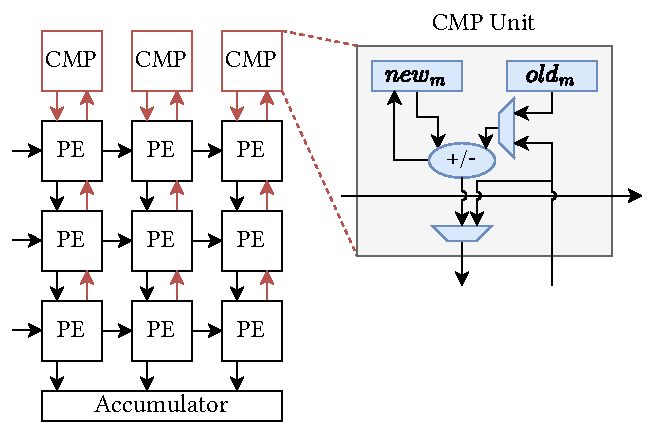
\includegraphics[scale=0.75]{figure_src/msaga.drawio.pdf}
  \caption{\MSAGA{}'s architectural modifications (highlighted in red) to the standard systolic array.}
  \label{fig:msaga-modifications}
  \Description{\MSAGA{}'s modifications.}
\end{figure}


\MSAGA{} is designed with two main goals:
(1) to reuse the systolic array's existing MAC units and dataflow to minimize hardware overhead;
and (2) to exploit the array's computational pattern to overlap multiple operations.


\autoref{fig:msaga-modifications} shows the architectural modifications to \MSAGA{}.
\MSAGA{} builds on the standard systolic array in \autoref{fig:systolic-array-example}
and introduces the following three key extensions to support non-matrix-multiplication operations in \FA{}.
First, \MSAGA{} introduces an upward data path, enabling column data streaming in both directions.
Second, it adds an array of comparators atop the MAC array to perform column-wise reductions on the fly.
Lastly, each PE is enhanced with the capability for linear interpolation, allowing it to perform non-linear
element-wise operations.



\subsection{Implementing \texttt{rowmax} on \MSAGA{}}

\begin{figure}[t]
  \centering
  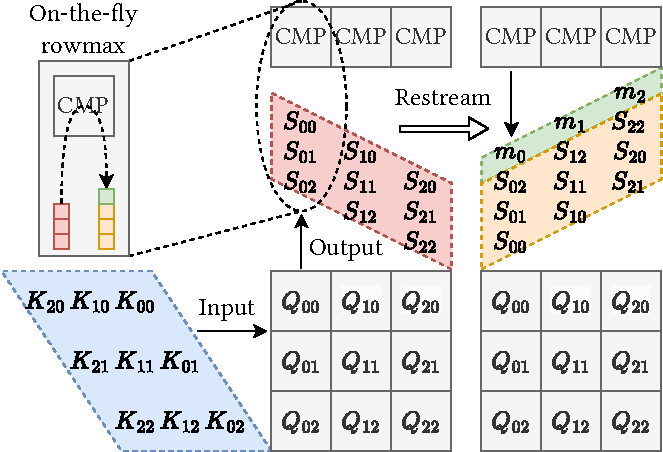
\includegraphics[scale=0.75]{figure_src/rowmax.drawio.pdf}
  \caption{On-the-fly \texttt{rowmax} generation.}
  \label{fig:rowmax}
  \Description{On-the-fly rowmax generation}
\end{figure}



To prepare for \texttt{rowmax}, \MSAGA{} first maps $Q$'s rows to the systolic array's columns, ensuring that rows of $S = QK^T$
(\autoref{line:mat1}, \autoref{alg:flash-attention}) are produced along the columns
of the array.
To compute $local_m = \texttt{rowmax}(S)$
(\autoref{line:rowmax-start}, \autoref{alg:flash-attention}),
\MSAGA{} uses the upward data path to stream each row of $S$ upward to a corresponding
comparator, which performs the maximum operation as a reduction of the entire row on the fly.

As shown in \autoref{fig:msaga-modifications}, each comparator consists of two registers
and a floating-point adder that supports addition, subtraction, and maximum operations.
The $old_m$ register stores the maximum row
value from the previous iteration, while the $new_m$ register keeps track of the
temporary row maximum for the current iteration, updated as each new row value arrives.
The comparator then re-streams each row value back into the systolic array after each $new_m$ update.
By the time the comparator completes the computation
$new_m = \max(local_m, old_m)$
(\autoref{line:new-m}, \autoref{alg:flash-attention}),
the corresponding row of $S$ is resident in the array.
\MSAGA{} then streams $new_m$ (highlighted in green) downward through the systolic
array to compute $N = S - new_m$ directly in place
(\autoref{line:s-minus-rowmax}, \autoref{alg:flash-attention}).



\subsection{Implementing \texttt{exp} on \MSAGA{}}

After \texttt{rowmax} and subtraction operations, an element-wise
exponential function is applied to the matrix $N$, illustrated in
\autoref{line:exp} of \autoref{alg:flash-attention}:
\[
P = exp\left(\frac{N}{\sqrt{d}}\right) =
exp2\left(\frac{\log_2 e}{\sqrt{d}} \cdot N\right).
\]
The constant element-wise multiplication on $N$
can be computed by streaming 
${\log_2 e} / {\sqrt{d}}$ 
from the left of the array as the multiplicand,
as $N$ is already resident in the systolic array 
after the subtraction.

We use \emph{piecewise linear interpolation} (PWL) to approximate the element-wise \texttt{exp2} operation~\cite{pwl}.
Inspired by~\cite{exp_pwl}, which calculates \texttt{exp2} of a fixed-point value, \MSAGA{} applies a similar scheme to decompose
a floating-point number 
$x$ into its integer and fractional components 
$x = x_i + x_f$, where $x_i$ is the integer part and $x_f$ is the fractional part. 
This decomposition leads to the identity:
\[
exp2(x) = 2^{x_i + x_f} = 2^{x_i} \cdot 2^{x_f}.
\]

As $N = S - \texttt{rowmax}(S)$, all elements in $N$ are less than or
equal to zero. Therefore $x_f \in (-1, 0]$, and consequently
$2^{x_f} \in (0.5, 1]$.
Given this limited range for $x_f$, we observe that an 8-piece uniform
PWL is sufficient to keep the relative error
around $10^{-2}$ in the final \FA{} results:
\[
exp2(x) \approx 2^{x_i} \cdot \left(slope_k \cdot x_f + intercept_k \right),
\quad k \in [0, 8),
\]
where the term $2^{x_i}$ only increases the exponent of the final result by $x_i$.

\begin{figure}[t]
  \centering
  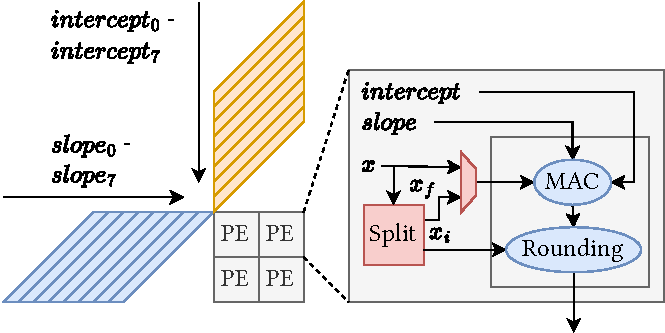
\includegraphics[scale=0.75]{figure_src/pe.drawio.pdf}
  \caption{Calculating \texttt{exp2} using PEs extended with PWL capability.}
  \label{fig:exp2-pe}
  \Description{\texttt{exp2} using piecewise linear interpolation.}
\end{figure}

As shown in \autoref{fig:exp2-pe}, the PWL
for $x_f$ can be implemented by reusing the MAC
units in the systolic array. A simple \textit{Split} unit
separates the input $x$ into its integer and fractional parts by shifting the mantissa
bits to align the exponent to zero.
To avoid storing linear interpolation coefficients in the systolic array, we stream $slope_k$
and $intercept_k$ values from the left and top of the array,
respectively.
We observe that all intercepts lie in the range $(0.5, 1]$,
so their exponent can only be $0$ or $-1$. The MSBs of their exponents
can be used to encode the interpolation index $k$.
This enables each PE to update its register based on $k$
without requiring additional control signals.


\subsection{Implementing \texttt{rowsum} on \MSAGA{}}


\begin{figure}[t]
  \centering
  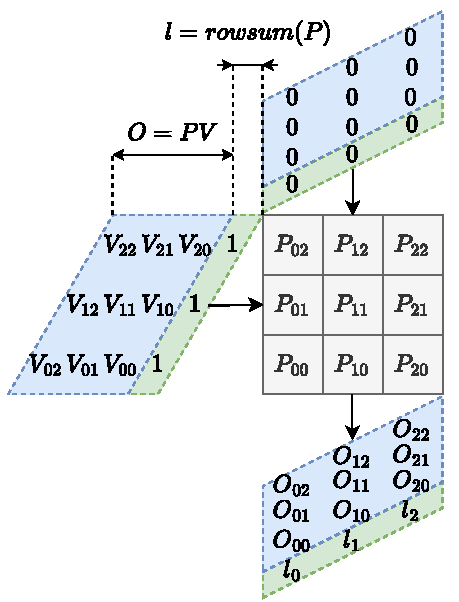
\includegraphics[scale=0.75]{figure_src/rowsum.drawio.pdf}
  \caption{Calculating \texttt{rowsum} using the systolic array.}
  \label{fig:rowsum}
  \Description{Implementation of \texttt{rowsum} using the systolic array.}
\end{figure}

As illustrated in \autoref{fig:rowsum}, the \texttt{rowsum} of $P$ is computed by
streaming a constant one from the left side of the array as the multiplicand,
and streaming zero from the top as the initial addend (highlighted in green).
The second matrix multiplication, $O = PV$
(\autoref{line:mat2}, \autoref{alg:flash-attention}),
can proceed concurrently along the downward data path (highlighted in blue),
starting just one cycle after the \texttt{rowsum} operation begins.
Once the intermediate results $local_l$ and $local_O$ exit the array from the bottom,
they are accumulated into the previous values $old_l$ and $old_O$ in the accumulator.
The updated $new_l$ and $new_O$ are then written back to the accumulation SRAM
(\autoref{line:l-acc} and \autoref{line:O-acc} in \autoref{alg:flash-attention}).



\subsection{Overlapping Computations with \SA{}}\label{sec:overlapping-computations}
\begin{figure*}[t]
  \centering
  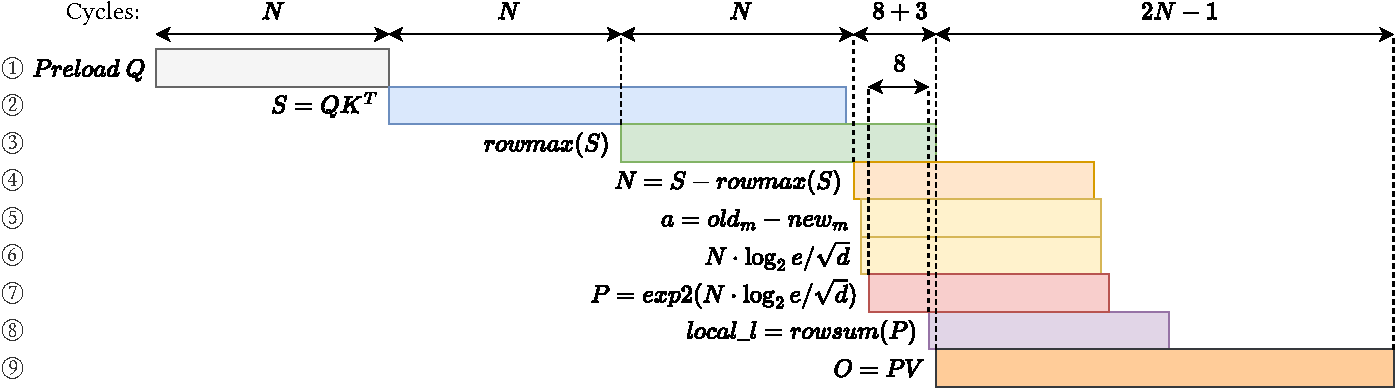
\includegraphics[scale=0.75]{figure_src/overlapping.drawio.pdf}
  \caption{Overlapped computations in \SA{} for the \FA{} inner loop.}
  \label{fig:overlapping}
  \Description{Overlapping computations in the systolic array.}
\end{figure*}

So far, we have introduced the key operations required to perform
\FA{} within a systolic array, including \texttt{rowmax}, \texttt{exp2},
and \texttt{rowsum}.
We now present \SA{}, an optimized kernel that makes the best use of \MSAGA{} to
achieve efficient overlapping of these operations in a single \FA{} iteration.

\autoref{fig:overlapping} illustrates how \SA{} schedules an iteration of \FA{}'s inner loop.
After \circled{1} preloading $Q$ into the systolic array,
\SA{} performs \circled{2} the first matrix multiplication $S = Q K^T$.
It specifically streams the last column of $K$ into the systolic array first (\autoref{fig:rowmax})
to make the first row of $S$ come out first.
Immediately after the first value of $S$ enters the comparator,
\SA{} starts \circled{3} the \texttt{rowmax} calculation, which takes $N$ cycles to complete.
Apart from re-streaming $S$ back to the systolic array,
the comparator also streams $new_m$ downwards,
allowing \circled{4} $N = S - new_m$ to be performed in-place one cycle after $S$ values are made stationary.
Next, \SA{} streams \circled{5} $a = old_m - new_m$ from the comparator,
alongside \circled{6} the constant $\log_2 e / \sqrt{d}$ from the left, propagating $a$ to the accumulator and performing
the constant multiplication $N \cdot \log_2 e / \sqrt{d}$ in parallel immediately
after \circled{4}.
Once this multiplication completes in the top-left PE,
\SA{} initiates \circled{7} the \texttt{exp2} operation,
also starting from the top-left PE. After $k = 8$ cycles of PWL, the result $P = \texttt{exp2}(N \cdot \log_2 e / \sqrt{d})$
is available.
\SA{} then schedules \circled{8} the \texttt{rowsum} of $P$,
starting from the top-left PE, followed by \circled{9} the second matrix
multiplication $O = PV$, both proceeding along the downward data path.

Overall, with \SA{}, \MSAGA{} takes $5 N + 10$ cycles to process an $N \times N$ \FA{} tile.
In contrast, on a naive $N \times N$ systolic array,
the two independent matrix multiplications without any data reuse require up to $8N-2$ cycles
due to preloading and input/output delaying overheads
discussed in \autoref{sec:systolic-array-intro}.

The re-scaling operation in \autoref{line:re-scaling} of \autoref{alg:flash-attention}
is only performed once per outer loop.
It is executed using the accumulator after the second matrix multiplication
completes.
In our implementation, this re-scaling step takes $2N + 20$ cycles,
negligible compared to the inner loop execution time.









